\documentclass[10pt]{article}

\usepackage{SDUstyle}
\usepackage{tabularx}
\usepackage{array}
\usepackage{booktabs}
\usepackage{longtable}
\usepackage{enumitem}
\usepackage{float}
\usepackage{url}

\setlist[itemize]{itemsep=0pt, parsep=0pt, topsep=2pt, partopsep=0pt}
\setlist[enumerate]{itemsep=0pt, parsep=0pt, topsep=2pt, partopsep=0pt}

\fancyhf{}
\fancyhead[C]{深度学习 2026 期末作业}
\fancyfoot[C]{\thepage}
\setlength{\headwidth}{\textwidth}

\hypersetup{
    colorlinks=true,
    linkcolor=blue,
    urlcolor=red,
    citecolor=green
}

\newcommand{\methodname}{LOSVER-Light}
\newcommand{\modtag}{\texttt{\textless MOD\textgreater}}

\newcommand{\figuretodo}[3]{
\begin{figure}[H]
    \centering
    \fbox{
        \begin{minipage}{0.86\textwidth}
            \centering
            \vspace{0.7cm}
            \textbf{待制作图：#1}\\[0.3cm]
            \small #2
            \vspace{0.7cm}
        \end{minipage}
    }
    \caption{#1}
    \label{#3}
\end{figure}
}

\def\singlecover{
\begin{titlepage}
    \centering
    
\includegraphics[width=0.65\textwidth]{./imgs/njubig.jpg}
    \par\vspace{1.5cm}
    {\Huge \heiti 深度学习 \par}
    \vspace{0.8cm}
    {\Large \heiti 2026 期末课程报告 \par}
    \vspace{1.2cm}
    {\LARGE \heiti 基于行级风险信号的轻量级函数漏洞检测方法研究：以 LOSVER-Light 为例 \par}
    \vspace{4.2cm}

    \begin{center}
        {\Large
        \makebox[4em][s]{\heiti 姓名}:\underline{\makebox[15em][c]{\heiti 高祯禧}}\\
        \makebox[4em][s]{\heiti 学号}:\underline{\makebox[15em][c]{\heiti 522025320036}}\\
        }
    \end{center}

    \vfill
    \today
\end{titlepage}
}

\begin{document}
\pagenumbering{Roman}
\setcounter{page}{0}
\singlecover

\setcounter{page}{1}
\thispagestyle{empty}
\section*{摘要}
\addcontentsline{toc}{section}{摘要}

漏洞检测是深度学习赋能软件工程的重要任务。近年来，代码预训练模型和大语言模型被广泛用于函数级漏洞检测，但函数级二分类仍存在两个问题：一是输入片段缺少跨函数和项目级上下文，二是模型可能依赖函数长度、危险 API、指针操作等浅层模式，而不是真正理解漏洞语义。本文参考 ASE 2025 论文 LOSVER 的行级信号思想\cite{nam2025losver}，设计并实现了一个轻量方法 \methodname。该方法先用静态规则为函数中的每一行计算风险分数，选取 top-k 风险行，再通过 \modtag{} 标签或风险行摘要将局部风险信号注入 Qwen2.5-Coder-1.5B 分类器\cite{hui2024qwen25coder}。实验在 CodeXGLUE Defect Detection / Devign 数据集上进行\cite{lu2021codexglue}。结果显示，\methodname{} Tag 在测试集上达到 F1=0.687276、ROC-AUC=0.760319、PR-AUC=0.757150，相比 Vanilla Qwen 分别提升 0.039916、0.073366 和 0.077507。消融实验表明 \texttt{top\_k=5} 是较合理的风险行数量。人工错例分析进一步说明，长函数、领域语义、错误处理和低层指针操作仍是当前方法的主要失败来源。

\newpage
\addcontentsline{toc}{section}{目录}
\tableofcontents
\newpage

\setcounter{page}{1}
\pagenumbering{arabic}

\section{引言}

软件漏洞会导致系统崩溃、权限提升、数据泄露和远程攻击，是软件工程中长期存在的重要质量问题。传统漏洞检测通常依赖静态分析、规则匹配、数据流分析和人工审计。这些方法可解释性较强，但在真实软件系统中容易受到语言特性、路径爆炸、调用关系复杂和误报率高等问题影响。随着深度学习和预训练语言模型的发展，研究者开始将代码看作一种特殊的程序语言文本，通过大规模代码语料学习 API 使用模式、控制流结构、错误处理习惯和潜在缺陷模式，从而辅助漏洞检测。

然而，漏洞检测并不是普通文本分类任务。一个函数是否存在漏洞，往往取决于少数关键代码行、边界条件、资源生命周期、调用者约束和项目级不变量。函数级漏洞检测数据集虽然便于训练和评估，却可能隐藏真实漏洞成因。模型只看到一个函数片段，却需要判断其中是否包含安全缺陷。在这种设置下，模型可能学习到一些表面相关模式，例如函数更长、危险 API 更多、指针更多、控制流更复杂，就更倾向于预测为漏洞。这类模式并非完全无用，但它们不等价于真正理解漏洞。

本文选择函数级漏洞检测作为“深度学习赋能软件工程”的具体任务，并以 ASE 2025 论文 LOSVER: Line-Level Modifiability Signal-Guided Vulnerability Detection and Classification 为主要参考\cite{nam2025losver}。LOSVER 的核心观点是：漏洞检测模型不应只被动读取完整函数，还应获得显式的行级信号，使模型更关注潜在脆弱代码区域。考虑到课程项目的时间和算力限制，本文没有完整复现 LOSVER 的 line-level modifiability localization 阶段，而是实现一个可复现、低成本的 \methodname{}：使用静态启发式规则近似行级风险信号，并将其注入 Qwen2.5-Coder 输入。

本文围绕四个研究问题展开。RQ1：显式行级风险信号是否能提升函数级漏洞检测性能？RQ2：不同信号注入形式是否影响效果？RQ3：简单代码度量基线能达到什么水平，是否揭示 benchmark 中的浅层模式？RQ4：风险行数量 top-k 是否存在信息量与噪声之间的折中？

本文的主要贡献有三点。第一，在课程作业可承受的算力范围内，将 LOSVER 的“行级信号引导”思想转化为一个端到端可运行的轻量系统，避免只停留在论文综述或概念复述。第二，设计了两种不同强度的风险信号注入方式，并与无提示的代码大模型、传统代码度量基线进行对照，使实验能够回答“提示是否有效”和“提示应如何组织”两个问题。第三，除主指标外，本文加入 top-k 消融和人工错例分析，尝试解释模型提升来自哪里、失败发生在哪里，以及函数级漏洞检测本身存在哪些不稳定因素。

\section{相关工作}

学习式漏洞检测通常将代码片段编码为向量，再通过分类器判断其是否存在漏洞。函数级二分类是最常见的实验设置，优点是数据构造和指标计算简单。但近两年已有研究反思这种设置的局限。ISSTA 2025 的 Top Score on the Wrong Exam 指出，许多 ML 漏洞检测工作把任务简化为“给定函数是否存在安全缺陷”的二分类问题，但真实漏洞往往依赖跨函数调用、配置、补丁历史和运行时环境，函数级标签可能让模型利用数据集偏差或 shortcut\cite{risse2025topscore}。

行级信号是本文最重要的方法来源。LOSVER 认为，漏洞检测模型应该由 line-level modifiability signal 引导，而不是完全依赖模型自己在完整函数中寻找重要位置\cite{nam2025losver}。与此相关，FSE 2025 的 Lost-in-the-End 研究了大语言模型在文件内漏洞定位中的位置敏感问题，说明输入组织方式会影响模型检测和定位能力\cite{sovrano2025lostend}。本文比较 Tag 和 Tag+Prefix 两种输入形式，正是为了分析风险行提示应保留在原始上下文中，还是应被提前汇总到输入开头。

另一类相关工作关注上下文不足。ISSTA 2025 的 Inter-procedural Semantic Completion 强调，许多漏洞无法只靠单函数判断，需要补充被调用函数、调用关系或跨过程语义\cite{wu2025vulnsc}。本文没有实现跨函数补全，而是明确将任务限制在函数级输入内，因此在结果分析中也承认：\methodname{} 可以突出函数内部可疑行，但无法恢复调用图、数据流切片和项目级状态。

此外，ICSE 2026 的 LLM-based Vulnerability Discovery through the Lens of Code Metrics 从代码度量视角分析 LLM 漏洞检测，指出模型预测可能与传统代码度量存在相关性\cite{weissberg2026metrics}。TSE 2025 的可解释漏洞检测研究则说明，仅输出二分类结果不足以支持开发者使用\cite{mao2025explainable}。本文因此加入 Metrics-Baseline、风险行触发原因和人工错例分类，使实验不仅报告分数，也分析模型可能依赖的浅层模式和失败原因。

\section{深度学习技术原理与方法}

本文使用的核心深度学习技术是代码语言模型微调。Qwen2.5-Coder-1.5B 是面向代码任务的预训练模型，能够将函数代码 token 编码为上下文表示\cite{hui2024qwen25coder}。在漏洞检测中，模型后接一个二分类头，输出函数为 vulnerable 的概率。由于全量微调 1.5B 参数模型成本较高，本文采用 4-bit QLoRA\cite{dettmers2023qlora}。QLoRA 将基础模型权重量化为 4-bit NF4 格式，并在训练时只更新 LoRA 低秩适配矩阵。LoRA 将权重更新近似为低秩分解，在冻结主体模型的同时学习任务相关增量参数，从而显著降低显存需求\cite{hu2021lora}，并适合在 $2\times$ RTX 3090 上完成训练。

从任务形式看，本文采用 sequence classification 范式。每个函数被序列化为一段输入文本，经过 tokenizer 转换为 token 序列后送入模型。模型最后输出两个类别的 logits，再通过 softmax 得到“安全”和“漏洞”的概率。训练时使用交叉熵损失，使漏洞样本的预测概率接近 1、安全样本接近 0。推理时并不直接采用默认 0.5 阈值，而是在验证集上搜索最优 F1 阈值，再固定该阈值评估测试集。这样做的原因是 Devign 的类别比例并非完全均衡，而且漏洞检测通常更关注 F1、Recall 与 Precision 的整体权衡。

\methodname{} 的流程分为四步。第一，对函数代码按行切分。第二，对每一行计算静态风险分数。第三，选择分数最高的 top-k 风险行并构造输入文本。第四，使用 Qwen2.5-Coder + QLoRA 训练函数级漏洞分类器。行级风险评分关注十类信号：敏感 API，如 \texttt{strcpy}、\texttt{memcpy}、\texttt{sprintf}、\texttt{malloc}、\texttt{free}；指针和数组符号，如 \texttt{->}、\texttt{*}、\texttt{[}、\texttt{]}；分支循环，如 \texttt{if}、\texttt{for}、\texttt{while}、\texttt{switch}；错误处理 token，如 \texttt{return}、\texttt{goto}、\texttt{NULL}；I/O 或系统接口，如 \texttt{open}、\texttt{read}、\texttt{write}、\texttt{recv}、\texttt{send}；此外还考虑长行、符号密度和未检查的敏感调用。所有候选行按风险分数降序、行号升序排序，默认选择 \texttt{top\_k=5}。

\begin{figure}[H]
    \centering
    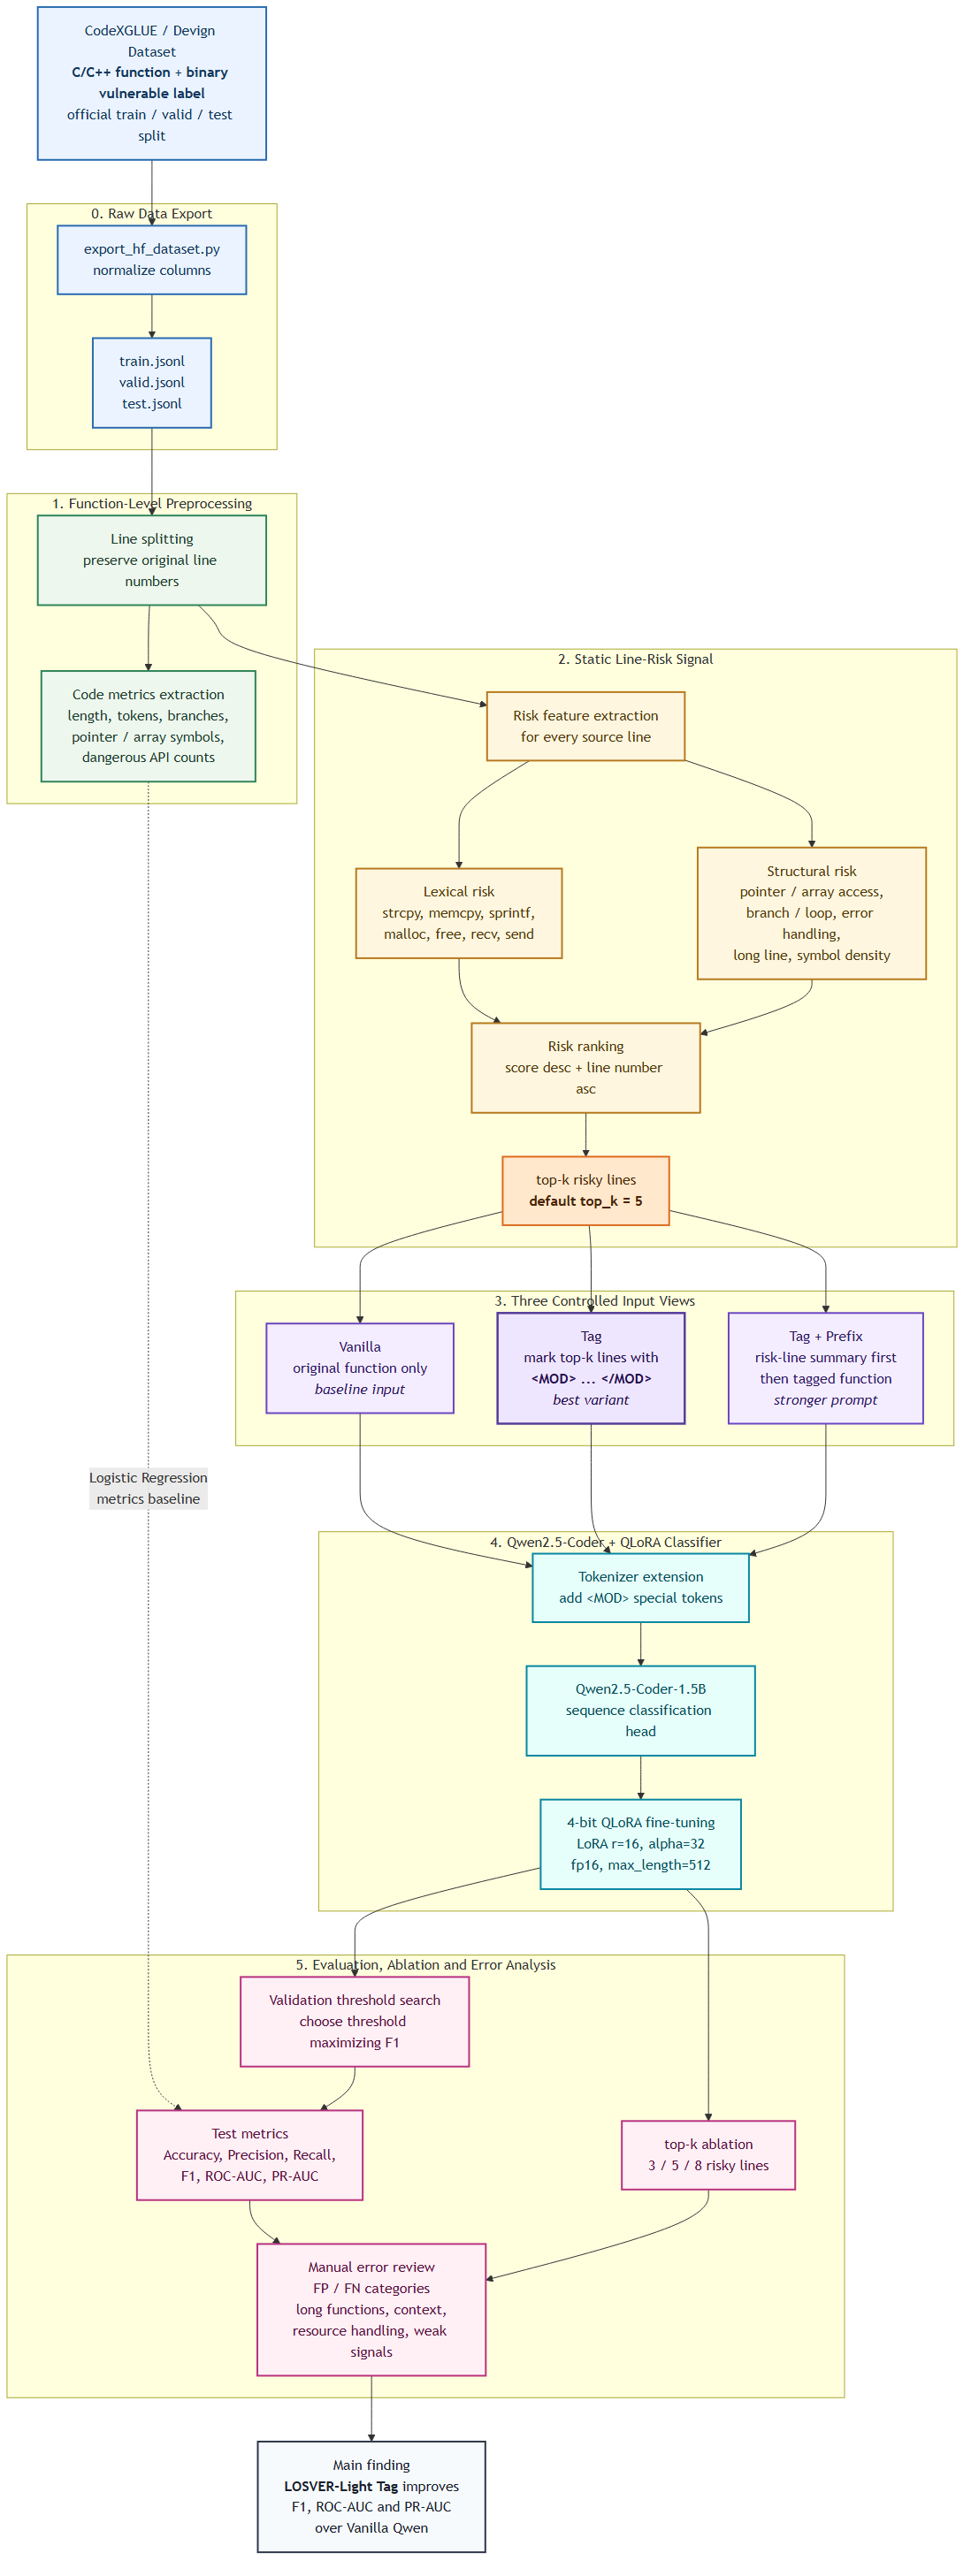
\includegraphics[width=\textwidth,keepaspectratio]{imgs/final/method_flow.png}
    \caption{LOSVER-Light 整体流程图}
    \label{fig:method-flow}
\end{figure}

基于风险行，本文构造三种输入。Vanilla 输入直接使用原始函数代码 \texttt{text\_vanilla}，作为现代代码大模型基线。Tag 输入在 top-k 风险行前后加入 \modtag{} 和 \texttt{\textless/MOD\textgreater}，形成 \texttt{text\_tag}，其优点是保留风险行在原函数中的上下文位置。Tag+Prefix 输入在 Tag 前添加风险行摘要，列出行号、分数、触发原因和代码内容，形成 \texttt{text\_tag\_prefix}，用于检验更强风险提示是否进一步提升检测效果。

这三种输入代表了不同的信息组织假设。Vanilla 假设预训练模型可以自己从完整函数中发现关键位置；Tag 假设模型需要轻量定位提示，但仍应结合原始上下文判断；Tag+Prefix 则假设模型在输入开头看到风险摘要后能更快聚焦重点。三者使用同一训练脚本和同一超参数，避免把输入格式差异与训练过程差异混在一起。由于 \modtag{} 标签是新增特殊标记，训练前会扩展 tokenizer 并同步调整模型词表，使模型能够学习这些标记在漏洞检测任务中的含义。

除深度模型外，本文还设计了 Metrics-Baseline。该基线从函数中提取 15 个代码度量特征，包括函数行数、非空行数、字符数、token 数、唯一 token 数、平均行长、最大行长、危险 API 数量、分支循环数量、指针数组符号数量、错误处理 token 数、符号密度、风险行数量、最大风险分数和平均风险分数，然后训练 Logistic Regression。这个基线用于判断浅层代码特征本身能达到什么水平。

\section{实验设计}

实验使用 CodeXGLUE Defect Detection / Devign 数据集\cite{lu2021codexglue}。该任务输入 C/C++ 函数，输出该函数是否存在漏洞。本文采用官方 train/valid/test 划分：训练集 21854 条，其中安全样本 11836 条、漏洞样本 10018 条；验证集 2732 条，其中安全样本 1545 条、漏洞样本 1187 条；测试集 2732 条，其中安全样本 1477 条、漏洞样本 1255 条。三个划分平均函数行数约为 110 行，中位数约为 57 行，说明数据中存在明显长函数长尾。

\begin{table}[H]
\centering
\caption{Devign 数据集划分与统计}
\label{tab:dataset-stats}
\begin{tabular}{lrrrrrr}
\toprule
Split & Samples & Safe & Vulnerable & Avg. Lines & Median Lines & Avg. Chars \\
\midrule
Train & 21854 & 11836 & 10018 & 109.57 & 57 & 3315.04 \\
Valid & 2732 & 1545 & 1187 & 109.55 & 57 & 3316.71 \\
Test & 2732 & 1477 & 1255 & 110.96 & 59 & 3371.97 \\
\bottomrule
\end{tabular}
\end{table}

数据预处理阶段首先导出原始函数和标签，再为每个函数生成代码度量特征、行级风险分数和三种文本输入。所有数据文件放在 \texttt{/mnt/sda/gzx/data/deeplearning2se}，模型缓存与训练输出放在 \texttt{/mnt/sda/gzx/models/deeplearning2se}，避免把大文件写入 Git 仓库。对风险行统计可以看到，许多函数只有少量明显高风险行，但长函数中风险行往往分布在多个控制分支或错误处理路径中。因此，本文没有简单把整段函数压缩为摘要，而是保留原始函数并在局部行上添加标记。

主实验比较四组方法：Metrics-Baseline、Vanilla Qwen、\methodname{} Tag 和 \methodname{} Tag+Prefix。三组 Qwen 方法使用相同骨干模型、相同训练参数和相同数据划分，只改变输入字段，因此它们的差异主要来自行级风险信号的注入方式。消融实验在 \methodname{} Tag 上比较 \texttt{top\_k=3/5/8}，用于分析风险行数量对结果的影响。

评价指标包括 Accuracy、Precision、Recall、F1、ROC-AUC、PR-AUC 和混淆矩阵。由于漏洞检测通常需要在漏报和误报之间权衡，本文不固定使用 0.5 阈值，而是在验证集上枚举 0.05 到 0.95 的阈值，选择 F1 最高者，再用于测试集。实验环境为 $2\times$ NVIDIA RTX 3090，Python 3.10，PyTorch 2.4.0，Transformers 4.48.0，PEFT 0.14.0，Accelerate 1.0.1，bitsandbytes 0.43.3。Qwen 训练使用 \texttt{max\_length=512}、epoch=3、per-device batch size=4、gradient accumulation=4、learning rate=$2\times10^{-4}$、fp16，随机种子为 42。

为了保证实验结论具有可比性，本文将所有 Qwen 实验都设置为相同训练轮数和 batch 配置，并使用验证集 F1 选择最终阈值。主实验关注不同输入形式的差异，消融实验只改变 \texttt{top\_k}，其他参数保持不变。这样的设计虽然不能覆盖所有超参数空间，但可以把核心变量控制在“是否加入行级信号”和“加入多少行级信号”上，更适合作为课程项目中的因果分析。

\section{实验结果与分析}

表 \ref{tab:main-results} 给出主实验测试集结果。\methodname{} Tag 取得最佳综合表现，F1=0.687276、ROC-AUC=0.760319、PR-AUC=0.757150。相比 Vanilla Qwen，它的 F1 提升 0.039916，ROC-AUC 提升 0.073366，PR-AUC 提升 0.077507，说明显式行级风险信号能够帮助模型更好地区分安全函数和漏洞函数。

\begin{table}[H]
\centering
\caption{主实验测试集结果}
\label{tab:main-results}
\begin{tabular}{lrrrrrr}
\toprule
方法 & Accuracy & Precision & Recall & F1 & ROC-AUC & PR-AUC \\
\midrule
Metrics-Baseline & 0.463397 & 0.461113 & \textbf{0.996813} & 0.630544 & 0.560892 & 0.536395 \\
Vanilla Qwen & 0.572108 & 0.520874 & 0.854980 & 0.647360 & 0.686953 & 0.679643 \\
\methodname{} Tag & \textbf{0.648243} & \textbf{0.580858} & 0.841434 & \textbf{0.687276} & \textbf{0.760319} & \textbf{0.757150} \\
\methodname{} Tag+Prefix & 0.608346 & 0.544493 & 0.901992 & 0.679064 & 0.756535 & 0.750676 \\
\bottomrule
\end{tabular}
\end{table}

\begin{figure}[H]
    \centering
    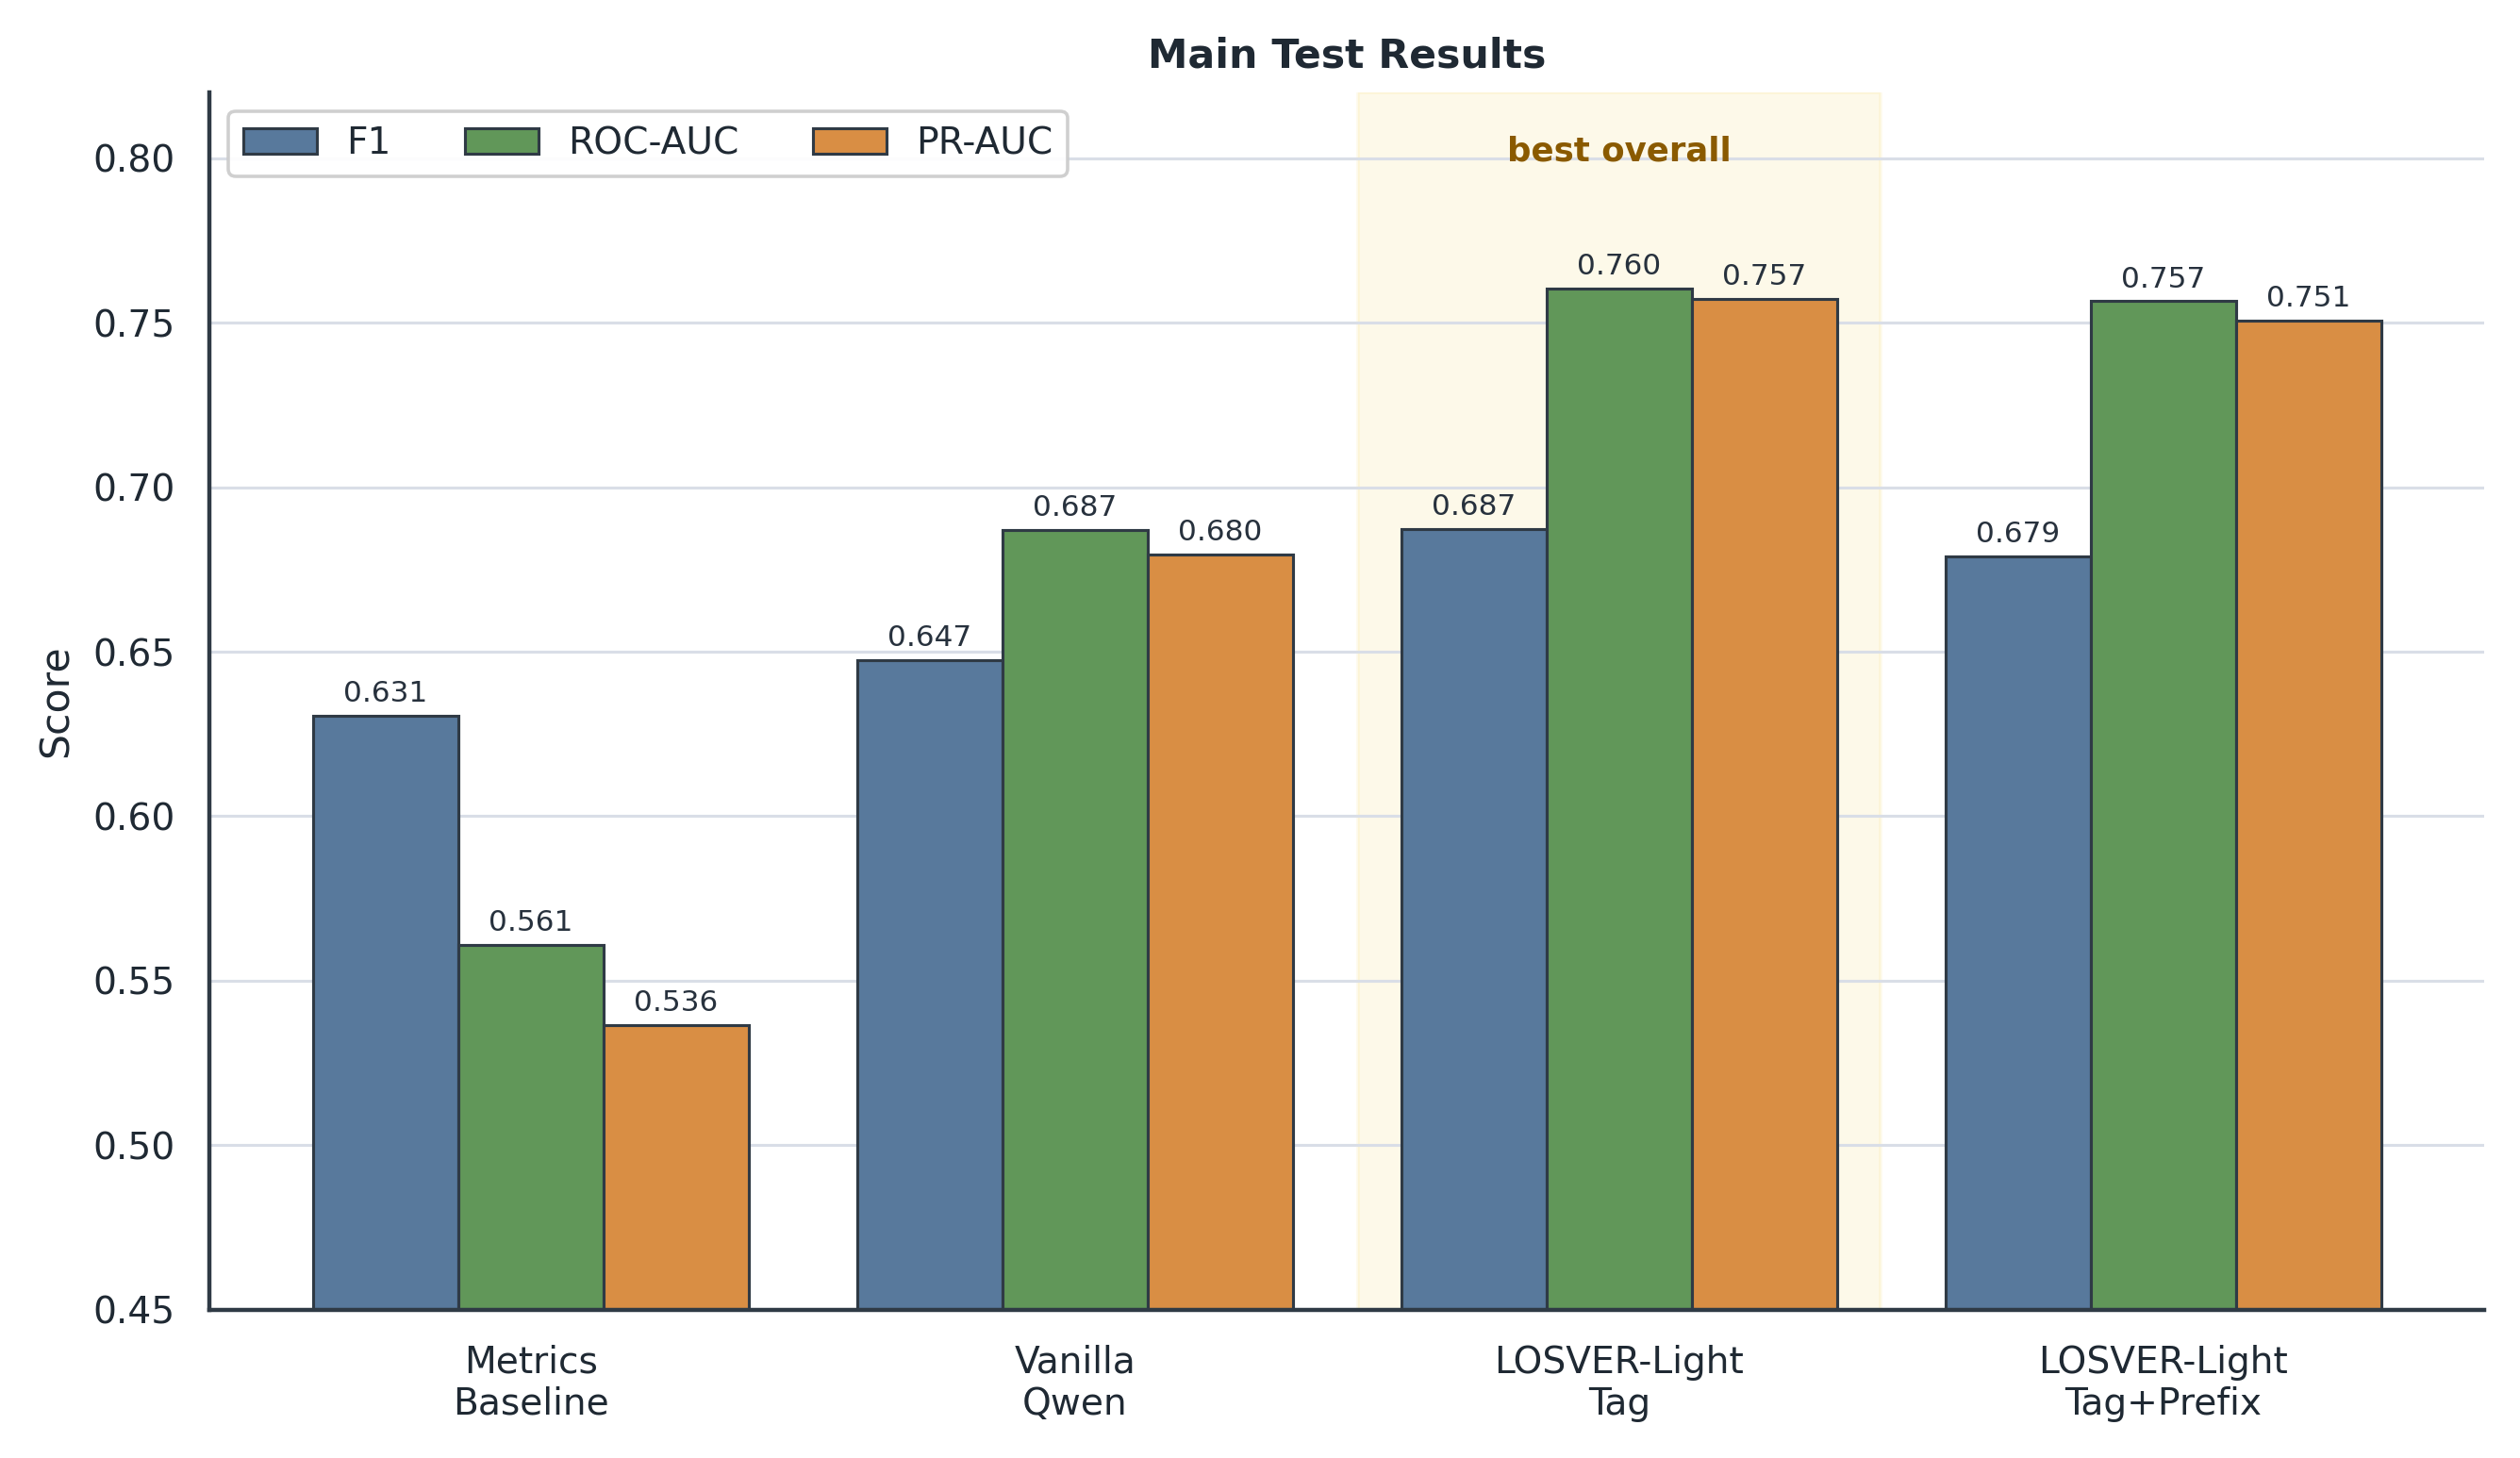
\includegraphics[width=0.9\textwidth,keepaspectratio]{imgs/final/main_results.png}
    \caption{主实验指标对比图}
    \label{fig:main-results}
\end{figure}

从混淆矩阵看，\methodname{} Tag 将 Vanilla Qwen 的 FP 从 987 降到 762，TN 从 490 提升到 715，说明 \modtag{} 标签主要改善了误报控制。Tag+Prefix 相比 Vanilla 也有提升，但没有超过 Tag。它的 Recall 达到 0.901992，高于 Tag 的 0.841434，但 FP 增加到 947，Precision 下降到 0.544493。这说明风险行摘要过于显式时，模型可能把启发式风险行理解为强漏洞证据，从而增加误报。相比之下，Tag 方式只在原始上下文中标记风险行，是更温和、更有效的注入形式。

Metrics-Baseline 的 F1 为 0.630544，看似接近 Vanilla Qwen，但 ROC-AUC 只有 0.560892，且 FP 高达 1462，只正确识别了 15 个安全函数。这表明代码度量确实可以捕捉一部分浅层漏洞信号，例如函数长度、危险 API 和指针访问，但区分能力很弱，尤其难以判断“看起来危险但实际安全”的底层系统代码。

表 \ref{tab:topk-ablation} 给出 top-k 消融结果。\texttt{top\_k=5} 在 F1、Accuracy 和 ROC-AUC 上表现最好。\texttt{top\_k=3} 的 Recall 降到 0.805578，说明风险行过少会遗漏关键上下文；\texttt{top\_k=8} 的 Recall 提升到 0.859761，但 Precision 降到 0.567298，说明更多风险行可以覆盖更多潜在漏洞位置，同时也会引入更多噪声。

\begin{table}[H]
\centering
\caption{top-k 消融实验结果}
\label{tab:topk-ablation}
\begin{tabular}{rrrrrrr}
\toprule
top\_k & Accuracy & Precision & Recall & F1 & ROC-AUC & PR-AUC \\
\midrule
3 & 0.644583 & \textbf{0.581703} & 0.805578 & 0.675576 & 0.755472 & 0.753953 \\
5 & \textbf{0.648243} & 0.580858 & 0.841434 & \textbf{0.687276} & \textbf{0.760319} & 0.757150 \\
8 & 0.634334 & 0.567298 & \textbf{0.859761} & 0.683560 & 0.758302 & \textbf{0.757988} \\
\bottomrule
\end{tabular}
\end{table}

\begin{figure}[H]
    \centering
    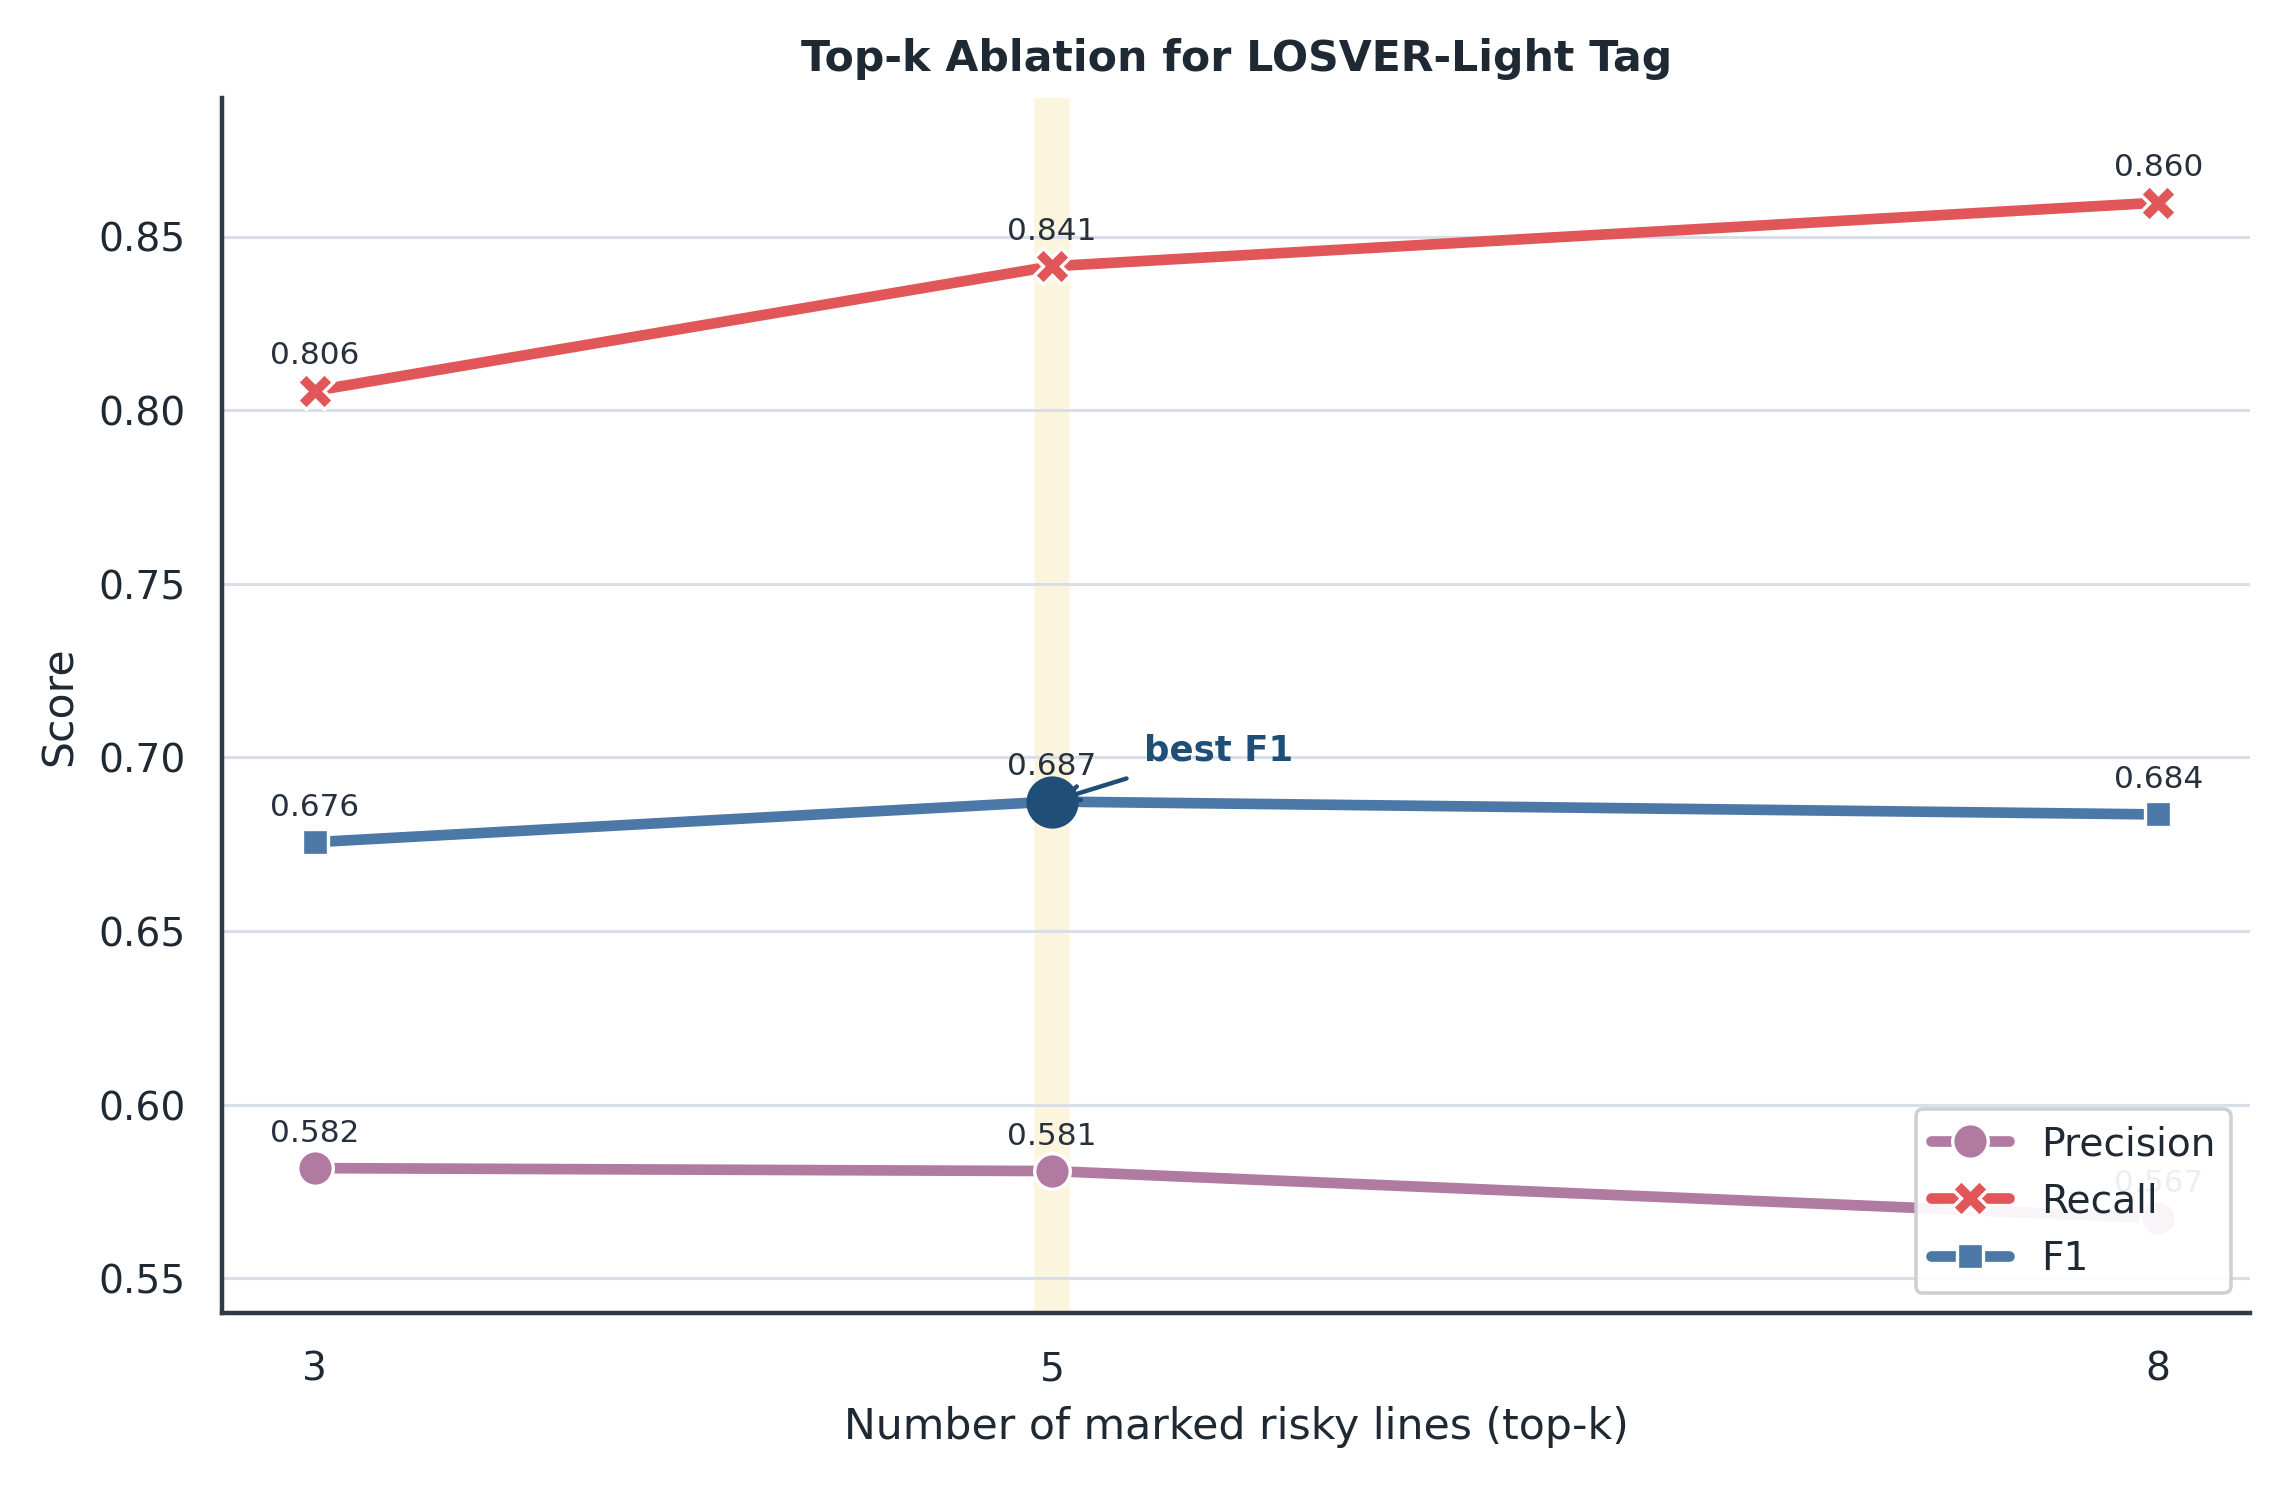
\includegraphics[width=0.82\textwidth,keepaspectratio]{imgs/final/topk_ablation.png}
    \caption{top-k 消融趋势图}
    \label{fig:topk-ablation}
\end{figure}

人工错例分析抽样检查了 24 个错误样本，其中包含 12 个漏报和 12 个误报。漏报主要来自长函数、领域语义依赖和弱行级信号，例如编解码器、页表遍历和虚拟机执行循环。误报主要来自错误处理、资源释放、I/O 解析、短包装函数和正常低层指针操作。这说明 \methodname{} 可以帮助模型聚焦可疑位置，但不能替代真正的跨行、跨函数和领域语义理解。

进一步看错例类别，\texttt{error\_or\_resource\_management\_false\_alarm} 出现 4 次，说明资源释放、错误返回和清理路径很容易被模型误认为漏洞；\texttt{long\_function\_or\_truncation} 出现 4 次，说明长函数仍会稀释或截断关键信息；\texttt{semantic\_or\_context\_dependent\_vulnerability} 出现 3 次，说明部分漏洞需要理解协议状态、调用约束或外部数据结构；\texttt{weak\_or\_misleading\_line\_signal} 出现 3 次，说明静态风险分数有时会把模型引向错误位置。这些结果与主实验一致：行级信号提升了模型平均性能，但它仍是启发式提示，而不是可靠的程序语义证明。

\begin{figure}[H]
    \centering
    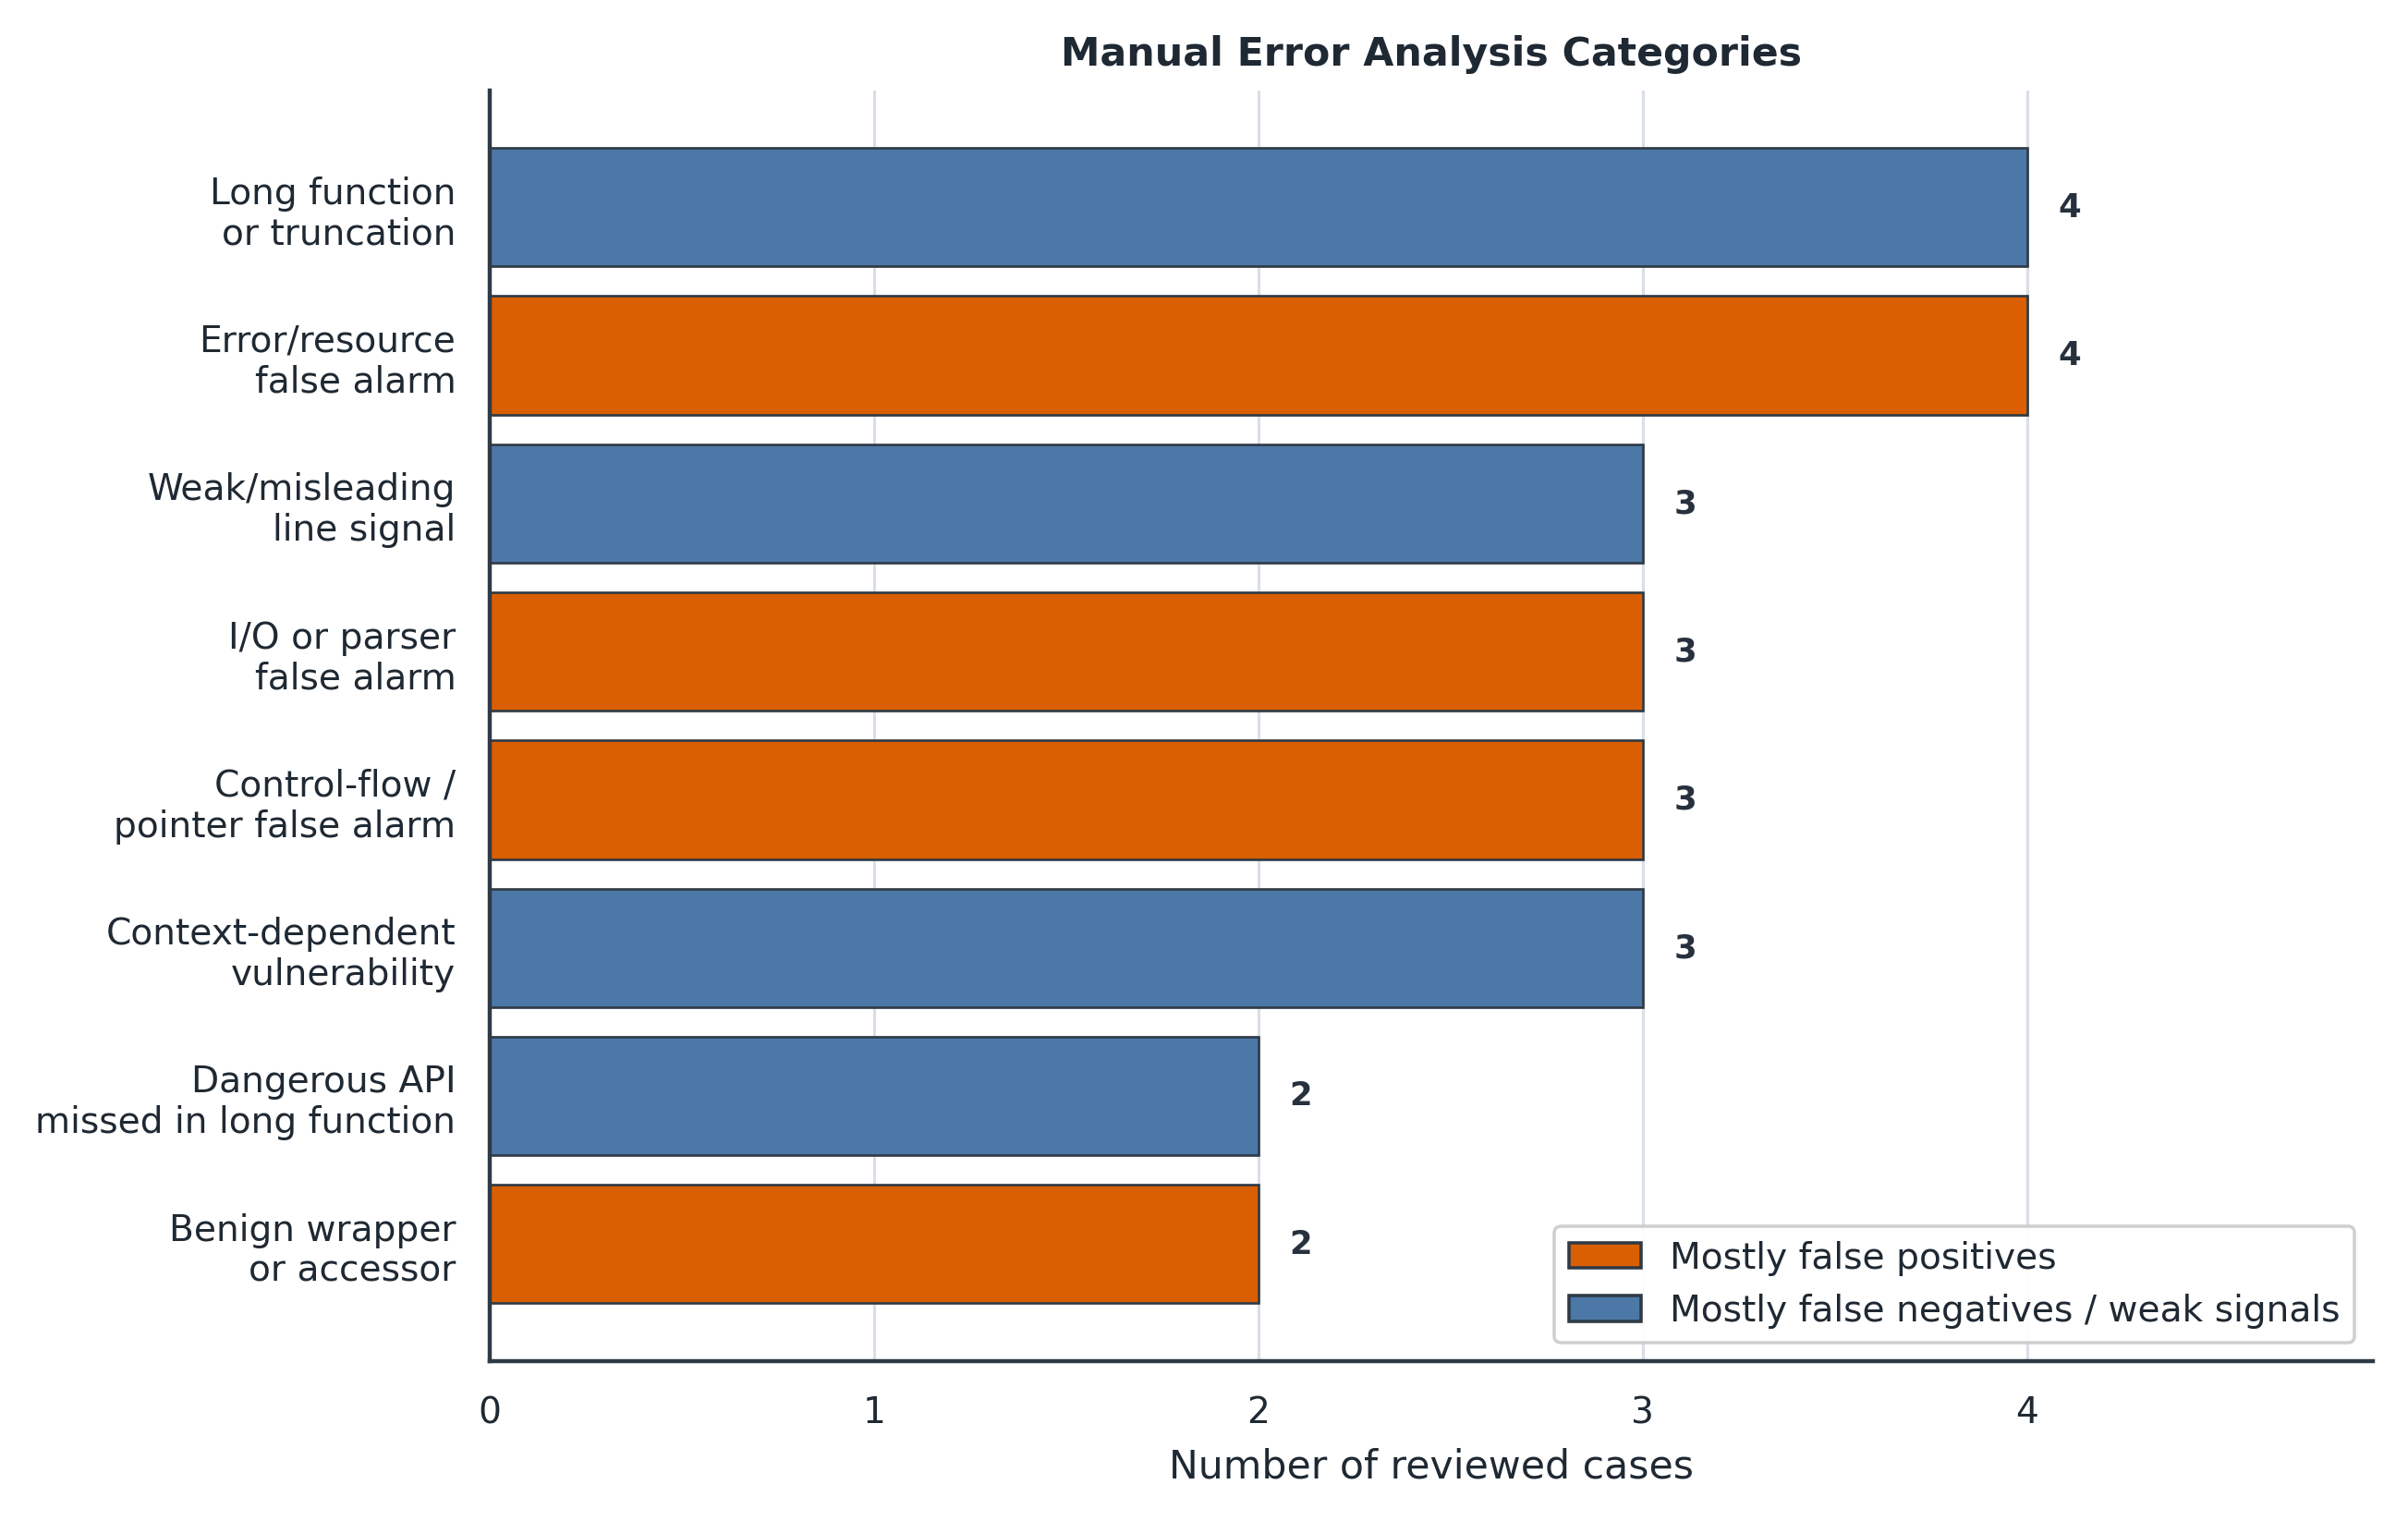
\includegraphics[width=0.88\textwidth,keepaspectratio]{imgs/final/error_analysis.png}
    \caption{人工错例类别分布图}
    \label{fig:error-analysis}
\end{figure}

从高分作业角度看，本文实验链条相对完整：先有传统代码度量基线，用于证明浅层模式确实存在；再有无行级提示的 Qwen 基线，用于衡量代码大模型自身能力；随后加入 Tag 和 Tag+Prefix，验证 LOSVER 思想的轻量实现；最后通过 top-k 消融和人工错例分析解释方法边界。相比单纯追求一个最高分数，这种设计更能体现深度学习软件工程实验中的可复现性、对照性和可解释性。

\section{局限性与未来工作}

本文存在五点局限。第一，\methodname{} 不是原始 LOSVER 的完整复现，静态风险评分不能等价于 line-level modifiability localization。第二，实验主要在 Devign 上进行，结果不能直接外推到真实工程漏洞发现。第三，主实验使用单一随机种子 \texttt{seed=42}，尚未进行多种子显著性检验。第四，静态规则可能把正常错误处理、资源释放、I/O 和指针操作误标为高风险。第五，\texttt{max\_length=512} 对长函数仍然有限，部分漏洞上下文可能被截断或稀释。

这些局限也构成了对实验结果的有效性威胁。内部有效性方面，行级风险规则由人工设计，可能偏向 C/C++ 中常见的内存安全模式，对逻辑漏洞、权限检查遗漏和并发问题覆盖不足。外部有效性方面，Devign 的函数级标签与真实漏洞发现流程存在差距，真实场景中开发者通常需要文件、调用链、补丁和运行环境信息。构造有效性方面，F1、ROC-AUC 和 PR-AUC 可以衡量分类能力，却不能完全衡量漏洞报告是否对开发者有用，因为开发者还关心可疑行定位是否准确、解释是否可信、误报排查成本是否可接受。

未来可以从五个方向改进：使用代码修改历史或弱监督标签训练学习式行级定位器；引入调用图、数据流切片或 inter-procedural semantic completion 补充跨函数语义；在 PrimeVul、Big-Vul 等数据集上做外部验证；使用多个随机种子报告均值、标准差和显著性检验；结合解释生成模型，让系统不仅输出漏洞概率，还输出可疑行和自然语言原因。

\section{结论}

本文围绕深度学习赋能软件工程主题，基于 LOSVER 的行级信号思想实现了轻量方法 \methodname{}，并在 Devign 函数级漏洞检测任务上完成了基线、主方法、消融和错例分析。实验表明，行级风险信号能够有效提升 Qwen2.5-Coder 的漏洞检测能力，其中 \methodname{} Tag 相比 Vanilla Qwen 在 F1、ROC-AUC 和 PR-AUC 上均有明显提升。消融结果说明风险行数量存在信息量与噪声之间的折中，\texttt{top\_k=5} 是较合理设置。代码度量基线和人工错例分析也表明，函数级漏洞检测中确实存在浅层模式，但仅靠这些模式无法可靠完成任务。总体而言，\methodname{} 证明了显式局部代码信号对代码大模型漏洞检测具有实际帮助，同时也说明真实漏洞检测仍需要更强的跨函数上下文建模和解释能力。

\bibliographystyle{IEEEtran}
\bibliography{references}

\end{document}
